\chapter{Desenvolvimento}

Algumas ferramentas foram fundamentais para o desenvolvimento deste projeto, a seguir descreverei as principais ferramentas utilizadas.

\section{Ferramentas utilizadas}

\subsection{VMWare Workstation Player}

Utilizado para executar máquinas virtuais \cite{vmware_player_ref}, no meu caso, com distribuições linux, Ubuntu\cite{ubuntu_ref} e Linux Mint\cite{linux_mint_ref}, para desenvolvimento do cliente e servidor C. Utilizei essa plataforma pela facilidade e confiabilidade necessárias para o desenvolvimento. O linux possui bibliotecas nativas que usei para compilação e execução do cliente e servidor.

\subsection {Eclipse}

Utilizado para escrita \cite{eclipse_ref}, em conjunto com o guia para windows \cite{devkit_windows_ref}, no embarcado. Com este tutorial, foi possível fazer o \textit{flash} de alguns projetos já existentes para teste do hardware em si.

\subsection{Putty}

Utilizado para ler as respostas do sistema embarcado, recebendo através da porta USB a resposta da execução do mesmo \cite{putty_ref}.

\subsection {SoAP UI}

Utilizado para testar a comunicação com o WebServer da empresa\cite{soap_ui_ref}.


\section{Projeto}

A partir do desenvolvimento de uma aplicação, que pode ser embarcada em um hardware modesto e utilizada com conexões precárias, em conjunto de diversos tipos de sensores visa-se atender este mercado de monitoramento e controle de ambientes. Assim, tratar-se-á, neste capítulo, sobre o desenvolvimento do projeto de cliente e servidor CoAP, em que é possível visualizar a implementação exposta no diagrama abaixo.

\begin{figure}[!htb]
	\centering
	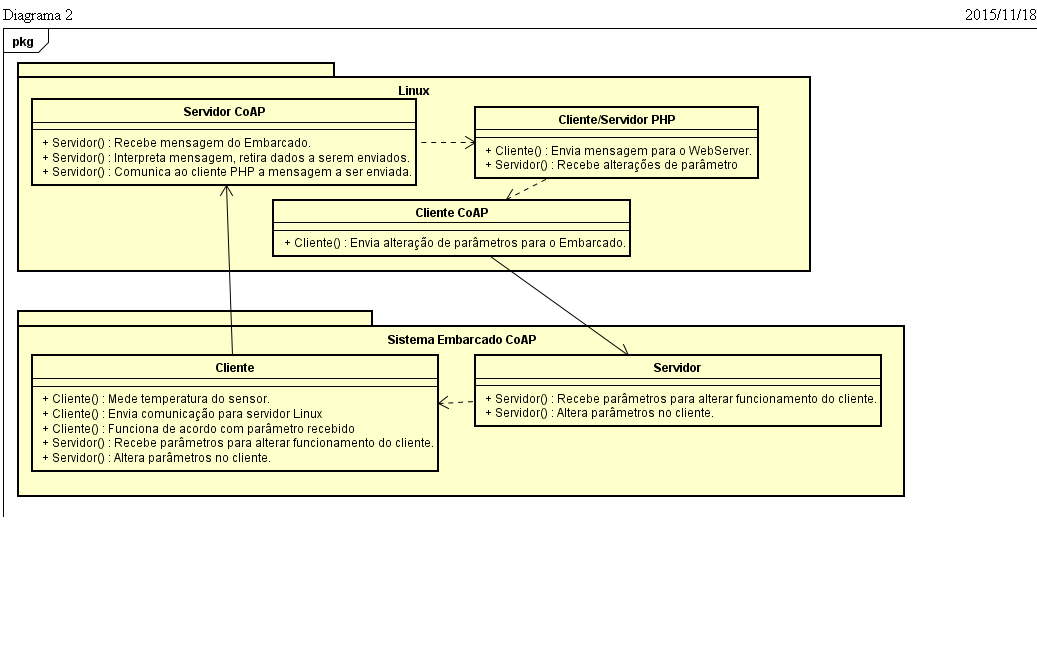
\includegraphics[width=1.0\textwidth]{../Diagrama_sem_webserver.png}
	\caption{Diagrama 1}
	\label{fig:Diagrama_lin_emb}
\end{figure}


Ainda que demonstrados cliente e servidor juntos, este projeto foi pensado e desenvolvido para ser utilizado de forma separada também. A implementação de ambos os elementos será descrita individualmente, e, por fim, será descrito o funcionamento delas em conjunto. Em mais detalhes, todo o código pode ser visto em \cite{cliente_servidor_coap}.

\section{Cliente CoAP}
O cliente foi desenvolvido em C, visando a aumentar a possibilidade de implantação em embarcados de baixo custo e melhoria de performance. A mensagem será transportada pelo protocolo UDP, utilizando o protocolo de aplicação CoAP. O funcionamento será dividido e descrito nas próximas seções para melhor entendimento.


\subsection{Conexão}
Como visto, utilizar-se-á o protocolo UDP para transporte, então, a conexão será feita, como demonstrada abaixo:

\begin{figure}[!htb]
	\begin{lstlisting}
	//CONEXAO
	int fd;
	
	struct sockaddr_in servaddr;
	fd = socket(AF_INET,SOCK_DGRAM,0);
	bzero(&servaddr,sizeof(servaddr));
	servaddr.sin_family = AF_INET;
	servaddr.sin_addr.s_addr = inet_addr("192.168.1.20");
	servaddr.sin_port = htons(7891);
	bind(fd,(struct sockaddr *)&servaddr, sizeof(servaddr));
	\end{lstlisting}
	\caption{Conexão do cliente, via porta 7891}
	\label{code:conexao_cliente}
\end{figure}

Ao ligar o socket à porta e ao endereço do servidor, via UDP, o envio da mensagem é feito da seguinte forma

\begin{figure}[!htb]
	\begin{lstlisting}
	if (rand()%100<PORCENTAGEM)
	{
	printf("\n\nEnviando\n\n");
	sendto(fd, buf_out, rsplen, 0, (struct sockaddr *) &cliaddr, sizeof(cliaddr));
	}
	else
	{
	printf("\n\nNão enviando, simulando erro de comunicação\n\n");
	}    
	\end{lstlisting}
	\caption{Simulação de erro de conexão}
	\label{code:simulacao_erro_conexao}
\end{figure}

Foi utilizada a função \texttt{if(rand()\%100<PORCENTAGEM)} para simular a perda de pacotes em conexões limitadas.


\subsection{Criação do pacote}

Foi usada a função \texttt{cria\_pkt }, e essa, por sua vez, chama a função  \texttt{monta\_header\_token} \ref{code:monta_header_token}, para criação do \textit{header} e \textit{token} do pacote, que são pré-definidos, no caso de o \textit{token} utilizado ser gerado pelo programa e não pelo usuário. Um pequeno trecho dela é visto na figura logo abaixo.

Foram empregadas também as funções \texttt{srand, rand()} para gerar aleatoriamente valores para o \textit{id} e para o \textit{token}, gerado de forma similar à utilizada para criar o \textit{id}, porém não foi transposta para o trecho abaixo.

\begin{figure}[!htb]
	\begin{lstlisting}
	void monta_header_token (coap_packet_t *pkt, uint8_t *token)
	{
		pkt->hdr.ver = 	 0x01; // versão 01;
		pkt->hdr.t = 	 0x00; // code 0 (confirmable);
		pkt->hdr.code =  0x02; //request -> 0000 0010 -> POST, 0000 0011 -> PUT
		srand(time(NULL));
		short int var_aux = rand()%254;
		pkt->hdr.id [0] = var_aux;
		short int var_aux = rand()%254;
		pkt->hdr.id [1] = var_aux;
		...
		pkt->tok.p = token;
		pkt->tok.len = strlen(token);
		pkt->hdr.tkl = pkt->tok.len;
	}
	\end{lstlisting}
	\caption{Pequeno trecho da função \texttt{monta\_header\_token}}
	\label{code:monta_header_token}
\end{figure} 

\subsection{Parâmetros}
\label{subsection:parametros}

Inicialmente, foi pensado em receber os parâmetros via linha de comando, passando-os como argumentos para a função, porém, além de dificultar os testes, posteriores à criação do cliente, pensou-se em fazer do cliente uma função do servidor. Para isso, uma mensagem padrão foi criada, com \textit{options} definidas e necessitando alterar apenas o \textit{payload}, com \textit{token} gerado de forma aleatória.
Como a função de identificação e verificação de parâmetros já havia sido feita para receber os parâmetros via linha de comando, apenas foi necessária uma adaptação da mensagem, para se encaixar nos moldes utilizados pela função padrão de recebimento de parâmetros; assim, a função seguinte de identificação não faz distinção entre o método empregado para envio de parâmetros utilizado.
A função utilizada para este fim, de alterar a mensagem pré-pronta deixando-a nos moldes da versão anterior, foi a \texttt{separa\_string}.

\subsection{Verificação e interpretação dos argumentos}

Aqui será utilizada parte da função \texttt{identifica\_arg} \ref{code:identifica_arg} para explicar como foi feita a identificação dos argumentos.

\begin{figure}[!htb]
	\begin{lstlisting}
	void identifica_arg (coap_packet_t *pkt, int argc, char **argv, char *buf_aux_opt_c, short int *buf_aux_opt_n)
	{
		...
		else if(strcmp(argv[j], "-op") == 0)
		{
			if (j+3 > argc) //caso não tenha os campos necessários
			{
				lida_erro_id(erro_argumento_num_option_invalido, argc, argv);
			}
			else if(veri_option (argv[j+1], argv[j+2]))
			{
				lida_erro_id(erro_argumento_num_option_invalido, argc, argv);
			}
			else
			{
				add_option(pkt, cont_aux, &buf_aux_opt_n[cont_op-1], argv[j+2], cont_op, &option_delta);
				j+=3;
			}
		}
		...
	}
	\end{lstlisting}
	\caption{Trecho da função \texttt{identifica\_arg} demonstrando a ação dela}
	\label{code:identifica_arg}
\end{figure}
\hfill \break
\hfill \break
\hfill \break
\hfill \break
\hfill \break
\hfill \break
\hfill \break
\hfill \break
\hfill \break
\hfill \break
\hfill \break

Como é possível ver na figura \ref{code:identifica_arg}, é feita uma verificação dos parâmetros, para averiguar se são argumentos válidos, com a função \texttt{veri\_option} e, caso sejam, sãoo adicionados ao pacote criado. A seguir, serão descritas, com mais detalhes, as funções \texttt{add\_token}, \texttt{add\_option} e \texttt{add\_payload}. 

\subsubsection{Funções de adicionar \textit{payload}, \textit{option}, \textit{token}}

Estas três funções \texttt{add\_token}, \texttt{add\_option} e \texttt{add\_payload} são utilizadas para adicionar o conteúdo da mensagem ao pacote, respectivamente, inserindo \textit{token}, \textit{options} e \textit{payload}. Elas têm funcionamento similar, copiando o conteúdo do buffer para o pacote e respeitando as especificações de tamanho da tabela \ref{table:valores_token_option_payload}.

\begin{table}[!htb]
	\centering
	\caption{Definições de tamanho para \textit{token}, \textit{option}, \textit{payload}}
	\label{table:valores_token_option_payload}
	\begin{tabular}{l|l}
		Tamanho máximo  & Valor em bytes \\ \hline
		Token tamanho   & 9              \\ \hline
		Option conteúdo & 24             \\ \hline
		Payload         & 64             \\ \hline
		Delta valor     & 64            
	\end{tabular}
\end{table}

\subsection{Monta pacote}

A mensagem é montada no pacote (\texttt{\&pkt}) e enviada através do buffer de saída (\texttt{buf\_out}). Essa tarefa é feita pela função \texttt{monta\_pkt}.
\begin{figure}[!htb]
	\begin{lstlisting}
	void monta_pkt (coap_packet_t *pkt, uint8_t *buf)
	{
		uint16_t running_delta = 0;
		char tempo[100];
		tempo_agora(tempo);
		...
		//Montando header
		buf[0] = (pkt->hdr.ver & 0x03) << 6;
		buf[0] |= (pkt->hdr.t & 0x03) << 4;
		buf[0] |= (pkt->hdr.tkl & 0xFF);
		buf[1] = pkt->hdr.code;
		buf[2] = pkt->hdr.id[0];
		buf[3] = pkt->hdr.id[1];
		p = buf+4;
		...
		//Montando token
		memcpy(p, pkt->tok.p, pkt->hdr.tkl);
		p = p+pkt->hdr.tkl;
		...
		//Montando options
		short int aux = (short int)pkt->numopts;
		for (i=0; i<aux; i++)
		{
			...
			memcpy(p, pkt->opts[i].buf.p, pkt->opts[i].buf.len);
			p = p + pkt->opts[i].buf.len;
		}
		...
		//Montando payload
		*p++ = 0xFF;
		memcpy(p, pkt->payload.p, pkt->payload.len);
		p = p+pkt->payload.len;
		
		//Adicionando tempo
		memcpy(p, tempo, (int)strlen(tempo));
		p=p+(int)strlen(tempo);
	}
	\end{lstlisting}
	\caption{Trecho da função \texttt{monta\_pkt} demonstrando a ação dela}
	\label{code:montar_pkt}
\end{figure}

É a função \texttt{monta\_pkt} também que faz o controle do parâmetro \texttt{running\_delta}, explicado na seção de opções do CoAP \ref{subsubsubsection{coap_option}}.

Ainda nela, é utilizada a função \texttt{tempo\_agora}, com objetivo de calcular o tempo no instante de execução. Através desse parâmetro, será calculado o desempenho do cliente. Abaixo será descrito, de forma simplificada, o funcionamento dessa função.

\verb||

\subsection{PUT}

A partir deste momento, a mensagem já foi montada, copiada para buffer e enviada, então, o cliente já está pronto e executando sua tarefa. 

Em caso de o tipo de mensagem ser PUT \ref{subsubsection:post}, o cliente já foi finalizado, necessitando apenas da função \texttt{separa\_string}, como discutido no tópico anterior Parâmetros \ref{subsection:parametros}, caso queira ser utilizada uma \textit{string} pré-definida para envio. O controle de tempo também é feito após o envio da mensagem e enviado para o arquivo de log.

\subsection{POST}

Para mensagens do tipo POST \ref{subsubsection:post}, foram utilizadas mais algumas funções adicionais: a  função de armazenar mensagem em buffer, \texttt{buffer\_msg} e a função para lidar com mensagem recebida \texttt{lida\_msg\_recebida}.

O tipo POST ainda realizará cinco tentativas de envio da mensagem, em caso de não recebimento do ACK.

\subsubsection{Separação de palavras}
A função \texttt{separa\_string} \ref{code:separa_string} tem objetivo de separar todos os parâmetros de uma \textit{string} única. Foi utilizado a variável \texttt{string\_sep}, que é alocada dinamicamente, conforme a \textit{string} que está sendo passada.

\begin{figure}[!htb]
	\begin{lstlisting}
	void separa_string (char **string_sep, char *buf, short int n_str, short int len)
	{
		for (i=0; i<len; i++)
		{
			if (buf[i] == ' ')
			{			
				string_sep[count_w][j] = '\0';
				count_w++;
				j=0;
			}
			else
			{
				string_sep[count_w][j] = buf[i];
				j++;
			}
		}
	}
	\end{lstlisting}
	\caption{Pequeno trecho da função \texttt{separa\_string}}
	\label{code:separa_string}
\end{figure}


\subsubsection{Buffer}

Esta função foi pensada para controlar o buffer, buscando uma posição vazia para armazenar a mensagem e escrevendo nesta posição do buffer. Ela também faz controle da capacidade do buffer, retornando uma mensagem de erro em caso de o buffer já estar cheio. Aqui poderia ser implementada outra forma de lidar com esse erro, a partir da reescritura sobre uma posição ocupada ou do descarte das mensagens para limpar o buffer após certo tempo. Um pequeno trecho da função é vista na figura \ref{code:buffer_msg}.

\begin{figure}[!htb]
	\begin{lstlisting}
	void buffer_msg (char *buf_out, char *buf_out_p, short int *cont_msg, short int *pos, char buf_str[][512])
	{
		int k, m, ult_esc = -1;
		if(*cont_msg > 7)
		{
			lida_erro_buffer (erro_buffer_cheio);
		}
		...
		else
		{
			k=1;
			while(k==1)
			{
				if(ult_esc == 7)
				{
					ult_esc = -1;
				}
				if(pos[ult_esc+k]==0)
				{
					...
					ult_esc++;
					*cont_msg = *cont_msg + 1;;
					pos[ult_esc] = 1;
					memcpy(buf_str[ult_esc], buf_out, 512);
					...
					break;
				}
			ult_esc++;
		}
	}
	\end{lstlisting}
	\caption{Pequeno trecho da função \texttt{buffer\_msg}}
	\label{code:buffer_msg}
\end{figure}

\subsubsection{Espera e reenvio da mensagem}

No caso de um POST, após a mensagem ser enviada, tem-se a espera pela resposta. Essa espera foi feita respeitando um parâmetro, o \texttt{NUM\_TIMEOUT}, que foi setado antes da execução, e é o limite máximo de tentativas que o cliente fará para envio da mensagem. É utilizada também a função \texttt{setsockopt} para fazer a espera pela mensagem por um período de tempo determinado pelos parâmetros \texttt{ACK\_WAIT\_TIMEOUT\_SEC} e \texttt{ACK\_WAIT\_TIMEOUT\_USEC}, respectivamente, a quantidade de segundos e micro-segundos em que o cliente esperará.

Então, recebida a mensagem, foi utilizada a função \texttt{lida\_msg\_recebida} para lidar com a mensagem do servidor que chega ao cliente, que seria a mensagem de ACK. E caso ela não seja recebida, a mensagem enviada deve ser reenviada. Conforme a figura \ref{code:envio_post}. 

\begin{figure}[!htb]
	\begin{lstlisting}
	while (num_timeouts < NUM_TIMEOUT)
	{
		if (setsockopt(fd, SOL_SOCKET, SO_RCVTIMEO,&tv,sizeof(tv)) < 0) 
		{
			perror("Error");
		}		
		else if (recvfrom(fd, buf_in, rsplen, 0, (struct sockaddr *)&cliaddr, &szcliaddr) >= 0)
		{
		
			if (1 == lida_msg_recebida (buf_in, buf_str, &cont_msg, pos, &time_post, &time_start, pFile))
			{
				num_timeouts = NUM_TIMEOUT;
			}			   		
		}
		else
		{
			printf("Entrando no msg não recebida, reenviando\n");
			if (rand()%100<PORCENTAGEM)
			{
				printf("\n\nEnviando\n\n");
				sendto(fd, buf_out, rsplen, 0, (struct sockaddr *) &cliaddr, sizeof(cliaddr));
			}
			else
			{
				printf("\n\nNot sending, simulando erro de comunicação\n\n");
			}
		}
	}
	\end{lstlisting}
	\caption{Pequeno trecho do cliente método POST}
	\label{code:envio_post}
\end{figure}

\subsubsection{Lida com mensagem recebida}

Essa função, \texttt{lida\_msg\_recebida} \ref{code:lida_msg_recebida} foi utilizada para comparar a mensagem recebida com a armazenada e para confirmar se é o ACK esperado. Caso a mensagem seja ACK, deve retornar 1, caso contrário, retornará 0.

Ela faz isso, comparando inicialmente o \textit{header} das duas mensagens, à armazenada e à recebida, e, entãom passa a comparar o restante da mensagem, até o final das \textit{options}.

\begin{figure}[!htb]
	\begin{lstlisting}
	int lida_msg_recebida (char *buf_in, char buf_str[][512], short int *cont_msg, short int *pos, struct timespec *time_post, struct timespec *time_start, FILE *pFile)
	{
		for (i=0; i<8; i++)
		{
			if (pos[i] == 1)
			{
				if (((buf_in[0] & (0xF0)) == 0x60) && ((buf_in[0] & 0X0F) == (buf_str[i][0] & 0x0F)) && ((buf_in[1] & 0xFF )== 0x44))
				{
					int cont = 0;
					for (j=0; j<(buf_in[0] & 0x0F); j++)
					{
						if(buf_in[2+j] == buf_str[i][2+j])
						{
							cont++;
						}
					}
					if (cont == (buf_in[0] & 0x0F))
					{
						pos[i] = 0;
						*cont_msg = *cont_msg - 1;
						memset(buf_str[i], 0x00, 512);
						return 1;
					}
				}
				else
				{
					return 0;
				}
			}
		}
	}
	\end{lstlisting}
	\caption{Pequeno trecho da função \texttt{lida\_msg\_recebida}}
\label{code:lida_msg_recebida}
\end{figure}

\hfill \break
\hfill \break
\hfill \break
\hfill \break
\hfill \break
\hfill \break
\hfill \break
\hfill \break
\hfill \break

Algumas funções adicionais também foram utilizadas, descritas de forma resumida.
As funções de \texttt{printf}, como, \texttt{printf\_header} ou \texttt{printf\_buffer}, têm função de imprimir o argumento que lhes é passado: são todas funções do tipo void que não fazem modificações no dado em si.
A função \texttt{tempo\_agora} recebe uma \textit{string}, e atualiza essa \textit{string} com o tempo no instante em que a função é chamada; ela é utilizada para adicionar o tempo à mensagem que será enviada.
A função \texttt{get\_time} recebe uma estrutura de tempo e a atualiza com o tempo no instante em que é chamada, sendo utilizada para calcular o tempo de execução do programa que foi salvo nos logs.
A função \texttt{calc\_time\_sub} foi utilizada para calcular a diferença de tempo, que é dada em segundos, desde um determinado tempo até o atual.
A função \texttt{corrige\_len} foi utilizada para corrigir o tamanho da mensagem: como a mensagem do servidor continha muitas sequências de 0, o cliente estava interpretando como se não fizesse parte da mensagem; essa função corrige o tamanho do buffer interpretado.
As funções de verificação, como \texttt{veri\_token}, fazem uma validação dos caracteres recebidos. Por exemplo, um campo de número de opção deve conter apenas números, um campo de nome da opção, pode conter números e letras, e assim por diante.
As funções de lidar com erros, por exemplo, \texttt{lida\_erro\_id}, foram separadas por função que atuam, ou seja, a do exemplo lida com erros na função \texttt{identifica\_arg}, gerando um código de erro que é definido antes da compilação, no código fonte do cliente.FAZER TABELA DE ERROS%

E assim, o cliente foi finalizado e ficou apto a enviar mensagens do tipo POST e PUT. O tipo de mensagem deve ser selecionado antes da compilação, alterando o parâmetro definido POST e PUT no início do código do cliente.

\section{Servidor}

O servidor foi planejado inicialmente para testar o cliente, e, após o desenvolvimento e a alteração do projeto, pensou-se em adicionar ele também ao sistema embarcado, para garantir certa flexibilidade do cliente. Já que, com o servidor embarcado, é possível fazer pequenas alterações no funcionamento do cliente, sem necessidade de refazer o \textit{flash} no embarcado.

O servidor, diferente do cliente, não foi feito do zero. Foi realizada algumas alterações no projeto \textit{microcoap} \cite{microcoap}. As modificações serão descritas a seguir, divididas por arquivo código alterado, o código completo se encontra na \cite{microcoap}. 

\subsection{Alterações na função \textit{main}}

As alterações na \textit{main} foram feitas para comportar o cliente como função do servidor. Essa tarefa foi feita utilizando a biblioteca \textit{pthreads}, podendo ser facilmente alterada para a função \textit{fork} caso necessário. Uma \textit{thread} ficará responsável pelo servidor, e outra \textit{thread} é encarregada do cliente. A função \texttt{rand} também foi utilizada no servidor, de maneira similar a do cliente, para, através do número aleatório gerado, enviar ou não a mensagem, simulando assim erro de pacotes. Nas figuras \ref{code:thread_serv_main_posix.c} e \ref{code:main_main_posic.c} é possível verificar alguns trechos da função \texttt{main\_posix.c}.

\begin{figure}[!htb]
	\begin{lstlisting}
	void *thr_func_serv_recv (void *arg)
	{
		fd_client = socket(AF_INET,SOCK_DGRAM,0);
		servaddr.sin_family = AF_INET;
		servaddr.sin_addr.s_addr = inet_addr("192.168.252.128");
		servaddr.sin_port = htons(PORT_CLI);
		while(1)
		{
			coap_packet_t pkt;
			n = recvfrom(fd_client, buf, sizeof(buf), 0, (struct sockaddr *)&servaddr, &len);
			...
			if (0 != (rc = coap_parse(&pkt, buf, n)))
				printf("Bad packet rc=%d\n", rc);
			...
			else
			{			
				coap_packet_t rsppkt;
				coap_handle_req(&scratch_buf, &pkt, &rsppkt);
				if (0 != (rc = coap_build(buf, &rsplen, &rsppkt)))
					printf("coap_build failed rc=%d\n", rc);
				else
				{
					
					if (rand()%100<PORCENTAGEM)
					{
						printf("\n\nSending\n\n");
						sendto(fd_client, buf, rsplen, 0, (struct sockaddr *)&servaddr, sizeof(servaddr));
					}
				}
			}
		}
	}
	\end{lstlisting}
	\caption{Pequeno trecho da \textit{thread} servidor da função \texttt{main\_posix.c}}
	\label{code:thread_serv_main_posix.c}
\end{figure}


\begin{figure}[!htb]
	\begin{lstlisting}
	int main(int argc, char **argv)
	{
		endpoint_setup();
		call_cli.tv_sec = get_var_time();
		call_cli.tv_nsec = 0;
		if ((rc = pthread_create(&thr[0], NULL, thr_func_cli, &call_cli)))
		{
			fprintf(stderr, "error: pthread_create, rc: %d\n", rc);
			return EXIT_FAILURE;
		}
		if ((rc = pthread_create(&thr[1], NULL, thr_func_serv_recv, &call_cli)))
		{
			fprintf(stderr, "error: pthread_create, rc: %d\n", rc);
			return EXIT_FAILURE;
		}
	}
	\end{lstlisting}
	\caption{Pequeno trecho da função \textit{main} da \texttt{main\_posix.c}}
	\label{code:main_main_posic.c}
\end{figure}

\hfill \break
\hfill \break
\hfill \break
\hfill \break
\hfill \break
\hfill \break

\subsection{Alterações na função \textit{endpoints}}

As principais alterações aqui foram a criação de novos métodos, que seriam utilizados para armazenar dados no servidor.

O método POST de temperatura (\texttt{temperature}) foi utilizado para armazenar a temperatura recebida, em um arquivo de log, e enviar de volta como resposta à temperatura armazenada. Já o método GET de temperatura apenas envia a última temperatura salva no servidor.

O método POST de tempo (\texttt{time}) foi utilizado para armazenar o último tempo enviado, que ditará a frequência de operação do cliente, ou seja, de quanto em quanto tempo a função \texttt{main\_posix} chamará o cliente.

A implementação dessas funções pode ser vista nos anexos.

Algumas funções adicionais foram utilizadas: como a função \texttt{set\_var\_time} para a \texttt{main\_posix} fazer alteração do tempo, quando receber um pedido de outro cliente; a função \texttt{get\_var\_time}, utilizada pelo próprio sistema, para chamar o cliente de acordo com esse tempo; a função \texttt{create\_var\_time}, utilizada para a criação inicial do tempo, setado por padrão no início do código fonte da função \texttt{endpoints.c}. E a própria função \texttt{endpoints\_setup}, que chama a função \texttt{create\_var\_time} para iniciar a função \texttt{endpoints}. Essas funções podem ser vistas na figura \ref{code:endpoints.c}.

\begin{figure}[!htb]
	\begin{lstlisting}
	void endpoint_setup(void)
	{
		build_rsp();
		variable = create_var_time ();
	}
	...	
	// Variável de tempo (usar no main-posix)
	void set_var_time (short int tempo)
	{
		variable.tempo = tempo;
	}
	short int get_var_time ()
	{
		return variable.tempo;
	}
	
	var_cli create_var_time ()
	{
		var_cli variable;
		variable.tempo = 5; //Segundos, para testes
		return variable;
	}
	\end{lstlisting}
	\caption{Pequeno trecho da função \texttt{endpoints.c}}
	\label{code:endpoints.c}
\end{figure}
